\documentclass[conference]{IEEEtran}
\IEEEoverridecommandlockouts
% The preceding line is only needed to identify funding in the first footnote. If that is unneeded, please comment it out.
\usepackage{cite}
\usepackage{amsmath,amssymb,amsfonts}
\usepackage{algorithmic}
\usepackage{graphicx}
\usepackage{textcomp}
\usepackage{xcolor}
\usepackage{tabularx}
\def\BibTeX{{\rm B\kern-.05em{\sc i\kern-.025em b}\kern-.08em
    T\kern-.1667em\lower.7ex\hbox{E}\kern-.125emX}}
\begin{document}

\title{Security of Electric Vehicle Charging Networks\\
}

\author{\IEEEauthorblockN{Nicholas Bennet}
\IEEEauthorblockA{\textit{Electrical and Computer Engineering} \\
\textit{New York University}\\
New York, USA \\
nb2831@nyu.edu}
\and
\IEEEauthorblockN{Danny Yuxing Huang}
\IEEEauthorblockA{\textit{Electrical and Computer Engineering} \\
\textit{New York University}\\
New York, USA \\
yh800@nyu.edu}
}

\maketitle

\begin{abstract}
Electric Vehicles adoption is increasing rapidly across the world including the USA. In this study we take a look at the various security risks which are posed by crowd sourced electric vehicle charging network apps and websites.
\end{abstract}

\begin{IEEEkeywords}
electric vehicles, charging network, security
\end{IEEEkeywords}

\section{Introduction}
The first modern all electric vehicle to be introduced to the USA was the Nissan Leaf in 2010. Since then electric vehicle adoption has been growing steadily from a mere 17,763 EVs sold in 2011 to 326,644 EVs sold in 2019. A total of 1,444,097 electric vehicles have been sold between 2011 and 2019 \cite{b1}. With this increasing adoption of electric vehicles multiple charging networks have come up all around the United States to fulfil the ever growing demand for Electric Vehicle charging stations. But this introduces a new problem as most of the apps and websites created by these charging networks only show charging stations of their network. To overcome this problem new crowd sourced apps were created which allowed users and manufactures to input details of charging stations as they were set up and also allowed users to update the details of these stations as the prices and number of plugs available changed. While some of these apps required a review by an authorized individual, some of the more popular apps don’t require any review before changes are published. We will look at the security issues this causes for an individual and the country as a whole. 

\section{Methodology}

\subsection{Searching for Apps and Websites}
To conduct the search for websites we used DuckDuckGo as the search engine. To automate the search we wrote a python program using the Selenium and BeautifulSoup libraries. The search terms used for this study are listed in ``Table. \ref{tab0}''. Duplicate links which were found in the list were removed by the program and the final list of websites was written to a csv file. The search was 5 pages deep as all of the relevant links were found in the first 5 pages. The relevant links in this case were defined as links which contained USA charging networks or recommendations for USA charging networks. As DuckDuckGo does get an approximate location information using a GEO::IP lookup most of the data related to the USA appear in the first few pages. The same search terms were then used to search for apps on Apple App Store.

\begin{table}[htbp]
\caption{Search Terms Used}
\begin{center}
\begin{tabular}{|l|}
\hline
\multicolumn{1}{|c|}{\textbf{Search Terms}} \\
\hline
EV charging\\
EV charging map\\
EV charging app\\
Electric vehicle charging\\
Electric vehicle charging map\\
Electric vehicle charging app\\
\hline
\end{tabular}
\label{tab0}
\end{center}
\end{table}

\subsection{Identifying editable attributes}
By looking at all the websites and apps which we gathered we created a list of all the attributes related to the charging stations that could be edited on the app and websites. We ended up with the list of editable attributes which is shown in ``Table. \ref{tab1}''. To determine which attributes were editable each website and app was opened and changes were attempted on each attribute. A record of the original value of each attribute was also kept. If the attribute was editable and no review was required, the attribute was reverted back to its original state as had been previously recorded. To ensure that the impact on the users was as minimal as possible several precautions were taken. At a given time only one attribute was edited for a particular charging station. If the address of the charging station was being changed it was changed only by one house number and immediately reverted back to the original as was recorded. If the price was being changed it was changed by one cent and was immediately changed back to the original value as recorded. All the edits were as minimal as possible and were performed between 12:00 AM to 02:00 AM local time for the charging station to reduce any chance of harm to a user. The attributes which do not require any review for making changes will be considered as truly editable for the purpose of this study.

\begin{table}[htbp]
\caption{List of Editable Attributes}
\begin{center}
\begin{tabular}{|l|}
\hline
\multicolumn{1}{|c|}{\textbf{Editable Attributes}} \\
\hline
Address                                          \\
Parking                                          \\
Plug Type                                        \\
Price                                            \\
Payment Types                                    \\
Amenities                                        \\
Operational Status                               \\
Timings                                          \\
Reviews                                          \\
Photos                                           \\
\hline
\end{tabular}
\label{tab1}
\end{center}
\end{table}

\subsection{Classification of websites and apps}
The websites and apps are also classified into three categories based on when they get their data from. First are the charging networks. These are the websites and apps created by the charging networks who install the charging stations and list their own charging stations. Second we have the data aggregators. These websites and apps aggregate and display data of charging stations from multiple charging networks and did not include data from the crowd sourced websites. Lastly we have the crowd sourced websites and apps. These websites and apps depend on their users and the charging networks to update the data they have on the various charging stations. The classification was very straightforward as we did not encounter any ambivalent cases. 

\subsection{Popularity of websites and apps}
We used three metrics to determine the popularity of websites and apps. While running the automated search script we also got multiple articles which recommended certain websites and apps. The number of mentions of a particular app or website in an article was used as the first metric to determine its popularity. For the purpose of this study an article is defined as a web page which contains verbiage recommending or listing certain charging network websites or apps. The article should also not be from the website or company which is recommended or listed in it. In the web search we also came across multiple sites which used plugins from certain websites to display charging network data on their websites. A plugin for the purpose of this study is defines as nested content provided by a certain website in the form of a code snippet which can be included in the code of another website to display data of charging networks. The number of times a plugin from a certain website was used was used as the second metric to determine popularity. Lastly the number of ratings and the number of ratings of apps on the Apple App Store was used as the third metric to determine its popularity.

\section{Limitations}
This study focuses on the security of charging networks in the USA. Any website, app or article which did not pertain to the charging networks in the USA were ignored for the purpose of this study. To check if a charging network website or app contained data of charging stations in the USA each website or app was checked to see if it listed any charging stations in the USA. Websites or apps which contained data of charging stations outside the USA along with the data of charging stations in the USA were also included.  This study also looks into apps present on the Apple App Store due to the unavailability of an android phone to search, download and test the apps available on Android. Certain websites which required either a subscription or purchase and registration of a vehicle to access the data on their charging networks were also ignored due to budgetary constraints.

\section{Identification of websites and apps}
This study focuses on the security of charging networks in the USA. Any website, app or article which did not pertain to the charging networks in the USA as mentioned before were ignored for the purpose of this study. This study also looks into apps present on the Apple App Store due to the unavailability of an android phone to search, download and test the apps available on Android. Certain websites which required either a subscription or purchase and registration of a vehicle to access the data on their charging networks were also ignored due to budgetary constraints.

\subsection{Search for websites and apps}
The automated search for websites using the python script yielded 874 links. After removing duplicate links from the same website we were left with 598 unique links. Out of these links we selected only the links pertaining to charging networks in the USA. We found 20 websites with charging network data, 17 articles recommending certain websites or apps and 20 websites that used plugins from other websites to display locations of charging stations.

\subsection{Classification of websites and apps}
Out of the 20 websites which were found containing data of charging networks, 3 were data aggregators, 9 were charging networks and 8 were crowd sourced websites(Fig.~\ref{fig1}). The websites in each category are listed in ``Table~\ref{tab2}''. In the 27 apps which were found in the Apple App Store, 5 were data aggregators, 13 were from charging networks and 9 were crowd sourced(Fig.~\ref{fig2}). The apps in each category are listed in ``Table~\ref{tab3}''.

\begin{table*}[htbp]
\caption{Charging Network Website Classification}
\begin{center}
\begin{tabular}{|l|l|l|}
\hline
\multicolumn{1}{|c|}{\textbf{Data Aggregator}} & \multicolumn{1}{c|}{\textbf{Charging Network}} & \multicolumn{1}{c|}{\textbf{Crowd Sourced}} \\
\hline
https://abetterrouteplanner.com/ & https://na.chargepoint.com/&https://www.plugshare.com/ \\
https://www.evtripplanner.com/planner/2-8/ & https://www.evgo.com/find-a-charger/ & https://afdc.energy.gov/fuels/electricity\_locations.html \\
https://evstationslocal.com/ & https://www.electrifyamerica.com/locate-charger/ & https://chargehub.com/en/charging-stations-map.html \\
 & https://blinkcharging.com/drivers/blink-map/ & https://openchargemap.org/ \\
 & https://voltacharging.com/drivers/ & https://evtripmap.com/ \\
 & \begin{minipage}[t]{0.5\columnwidth}%
https://www.ford.com/buy-site-wide-content/overlays/try-the-tech/ %
\end{minipage} & https://chargemap.com/map \\
 & \begin{minipage}[t]{0.5\columnwidth}%
https://charge.greenlots.com/evowner/portal/locate-charger %
\end{minipage} & https://www.google.com/maps/search/ev \\
 & https://tools.greencars.com/charging/ & https://www.evmatch.com/s \\
 & https://www.flo.com/drivers/map/ & \\
 \hline
\end{tabular}
\label{tab2}
\end{center}
\end{table*}

\begin{table*}[htbp]
\caption{Charging Network App Classification}
\begin{center}
\begin{tabular}{|l|l|l|}
\hline
\multicolumn{1}{|c|}{\textbf{Data Aggregator}} & \multicolumn{1}{c|}{\textbf{Charging Network}} & \multicolumn{1}{c|}{\textbf{Crowd Sourced}} \\
\hline
A Better Route Planner (ABRP) & Blink Mobile & Alternative Fueling Stations \\
Charge App: EV charging & ChargePoint & AmpUp - EV Charging \\
Chargeway & Electrify America & ChargeFinder: Public Charging \\
Go-Station EV Charging & EVCS & ChargeHub EV Map \\
RechargeNow & EVgo EV Chargers & Chargemap - Charging stations \\
 & EVolution | EV Network & EVmatch \\
 & FLO - EV Charging Network & Open Charge Map \\
 & Greenlots & Plug Map \\
 & Greenspot EV Charging & PlugShare \\
 & PowerFlex &  \\
 & SemaConnect & \\
 & Volta Charging &  \\
 & Xeal & \\
\hline
\end{tabular}
\label{tab3}
\end{center}
\end{table*}

\begin{figure}[htbp]
\centerline{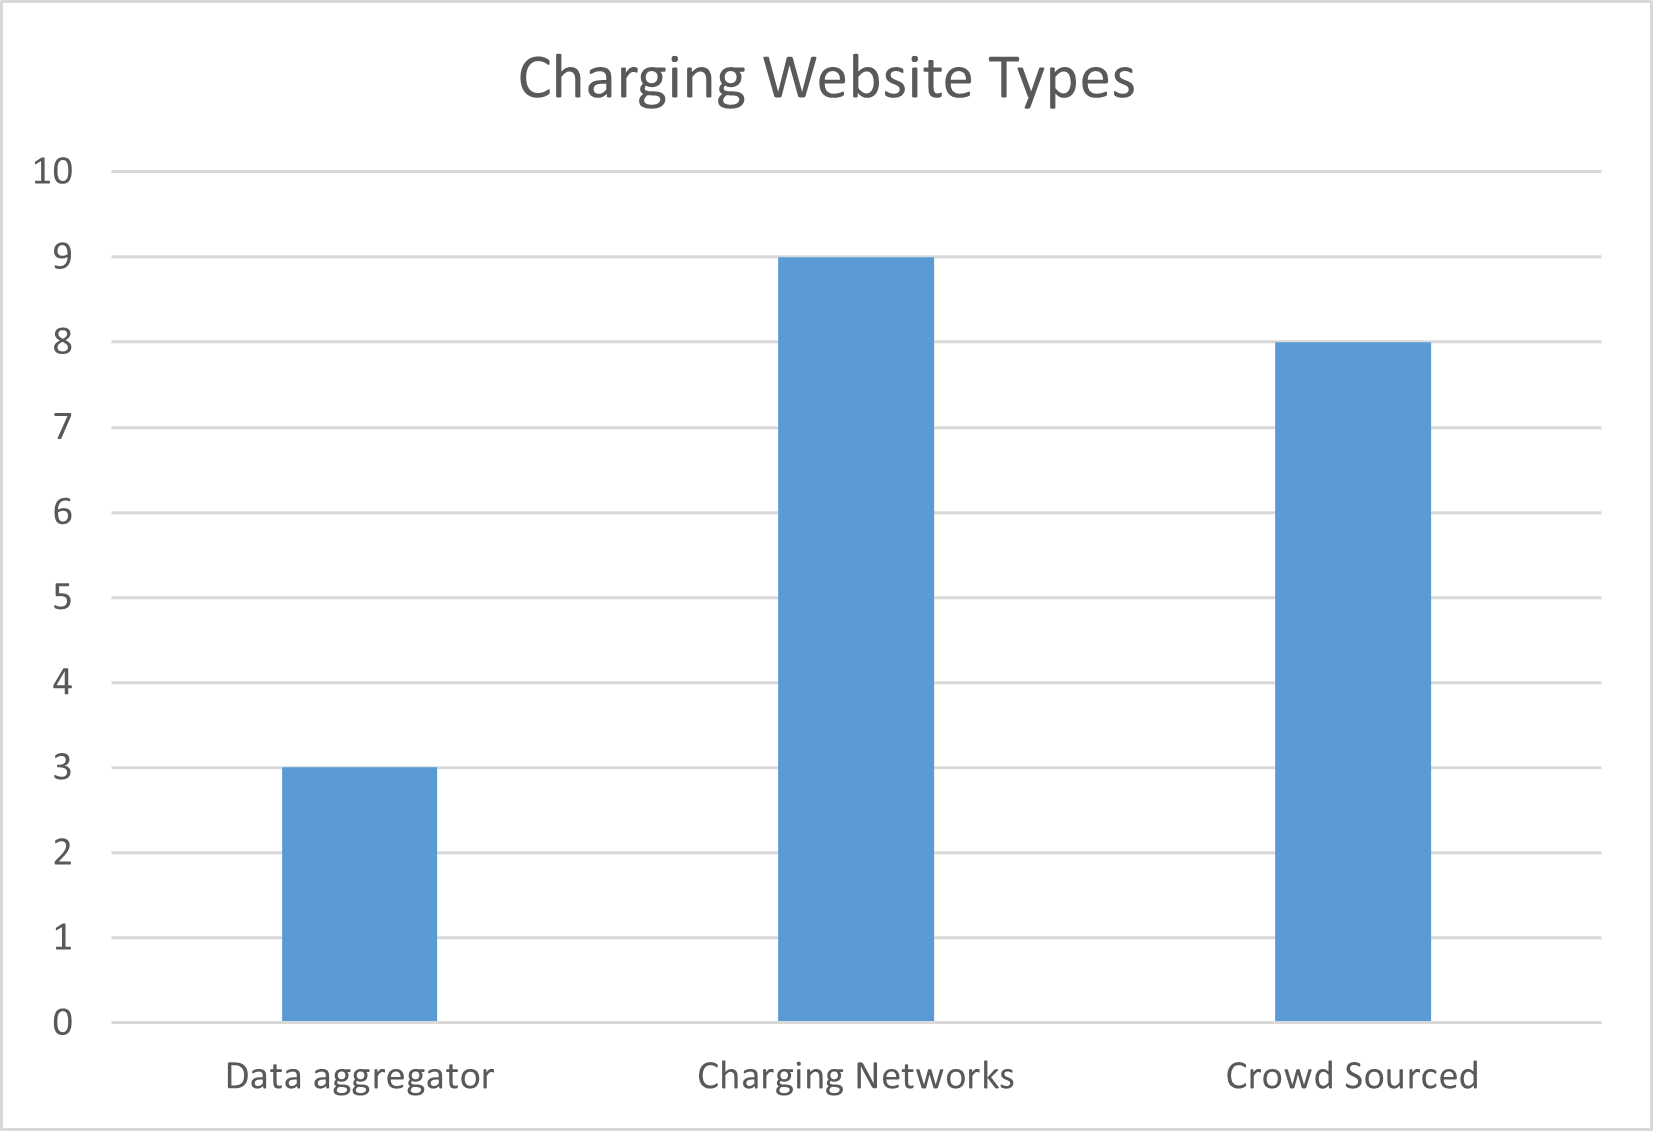
\includegraphics[width=\columnwidth]{Picture1.png}}
\caption{Charging Website Types}
\label{fig1}
\end{figure}

\begin{figure}[htbp]
\centerline{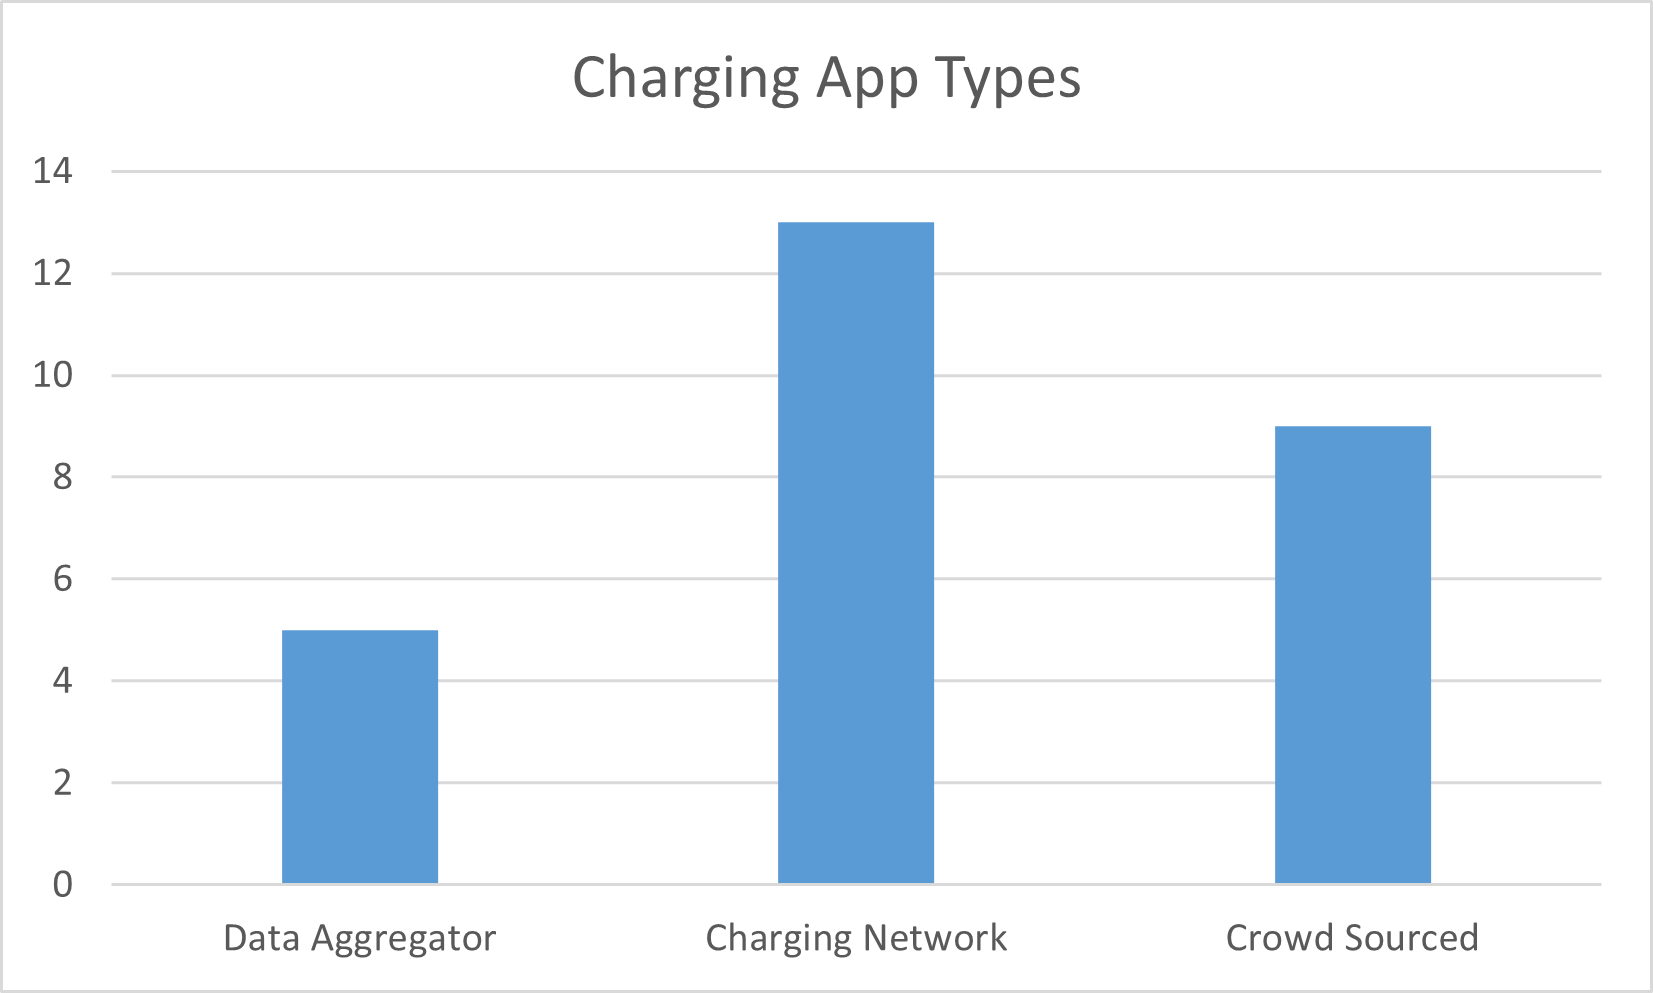
\includegraphics[width=\columnwidth]{Picture2.png}}
\caption{Charging App Types}
\label{fig2}
\end{figure}

\subsection{Editable attributes}
Out of the 8 apps which were crowd sourced at least 2 apps with attributes which were truly editable(Fig.~\ref{fig3}). In the case of apps we had 1 app for each attribute which was truly editable(Fig.~\ref{fig4}).

\begin{figure}[htbp]
\centerline{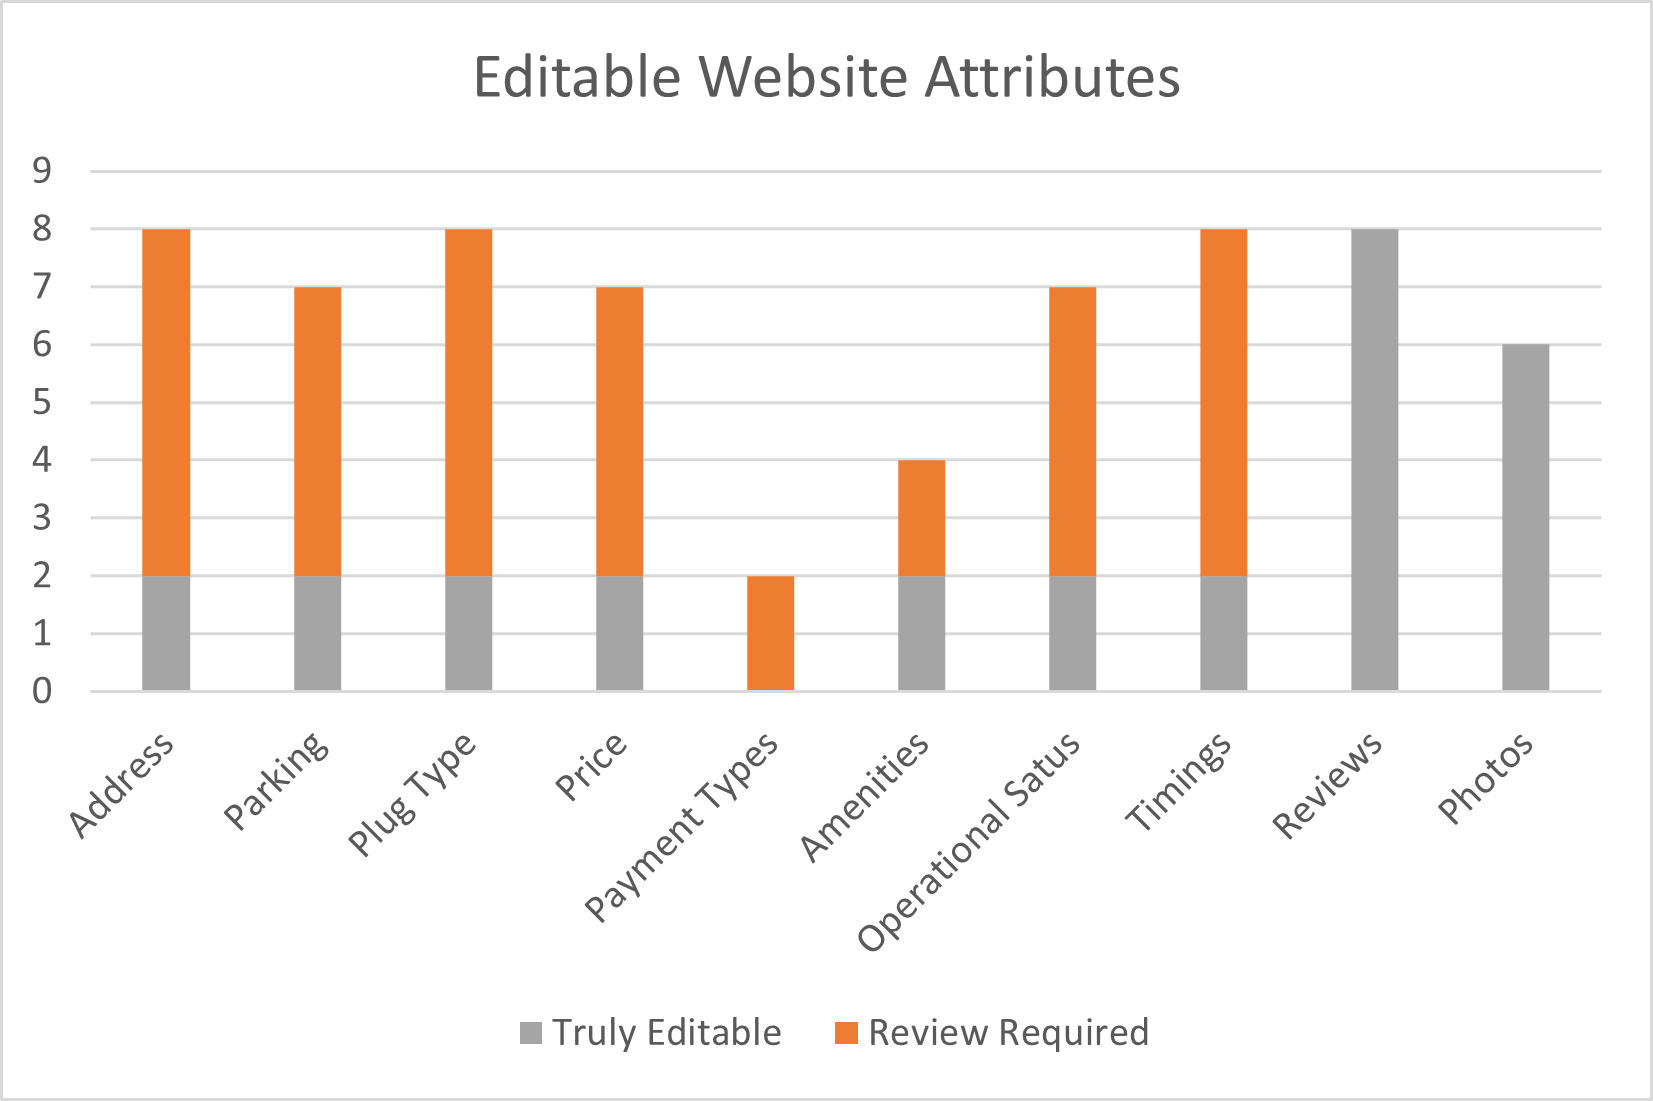
\includegraphics[width=\columnwidth]{Picture3.png}}
\caption{Editable Website Attributes}
\label{fig3}
\end{figure}

\begin{figure}[htbp]
\centerline{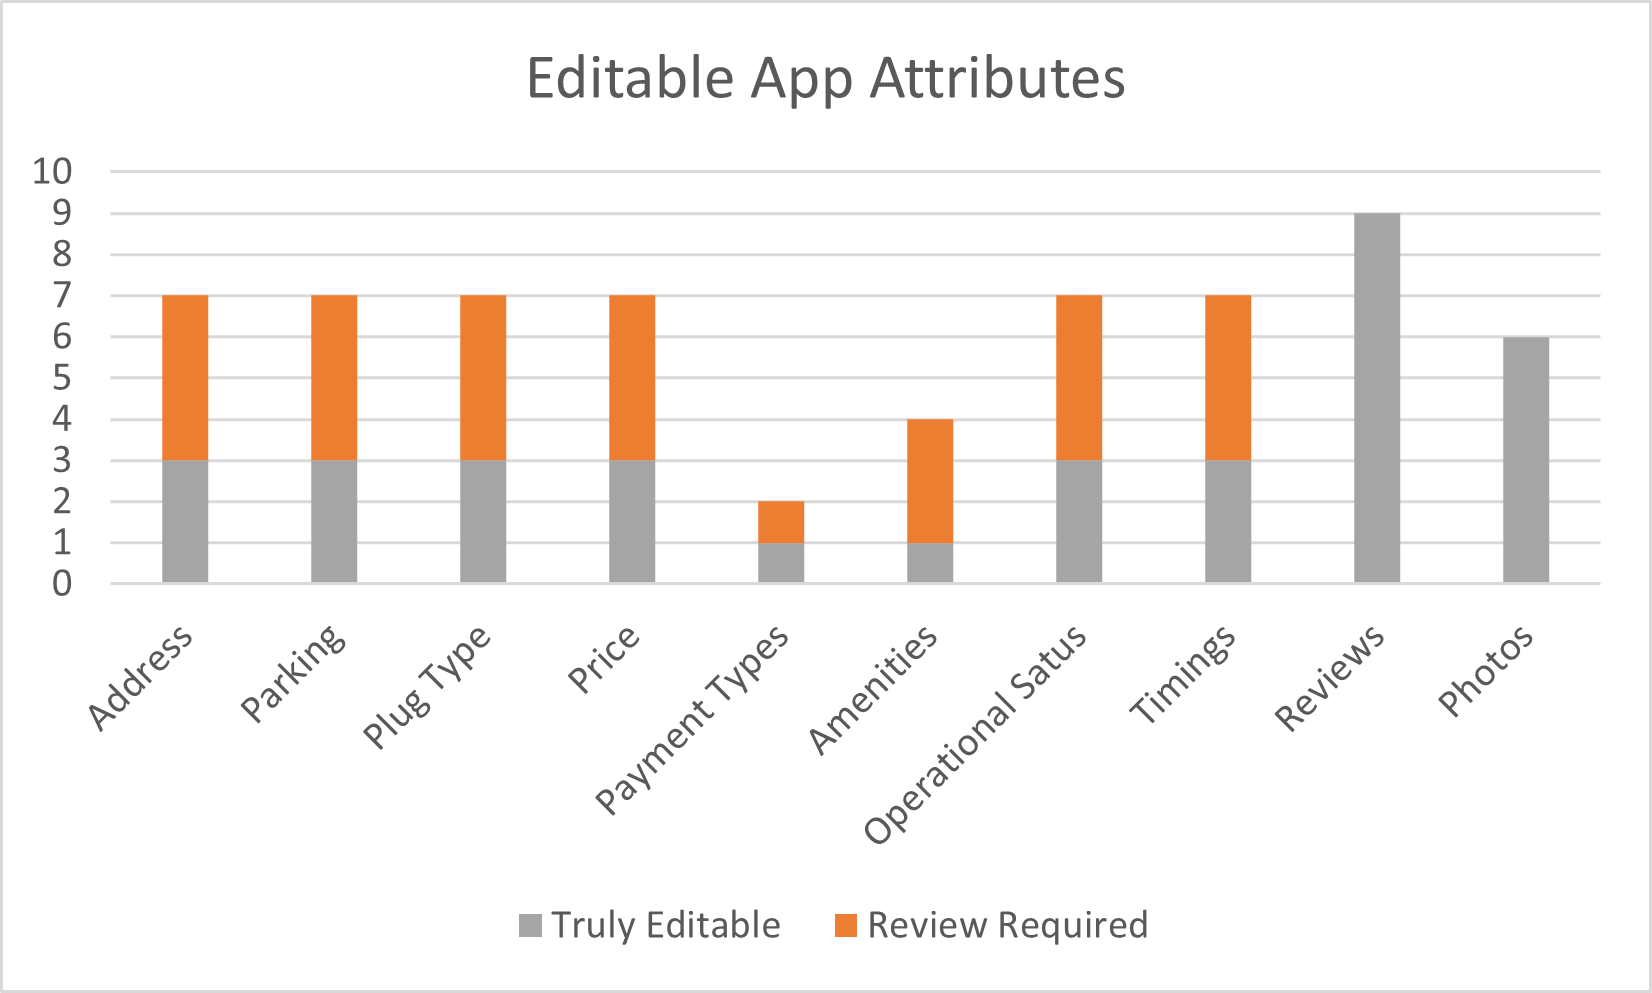
\includegraphics[width=\columnwidth]{Picture4.png}}
\caption{Editable App Attributes}
\label{fig4}
\end{figure}

\section{Popularity of websites and apps}
It is important to judge the popularity of the websites and apps as it gives USA an insight into how serious the issue at hand is by letting USA know which website or app is more frequented by users.

\subsection{Popularity in articles}
Out of the 17 articles which were found in the web search, PlugShare was the most popular and was mentioned in 16 of the articles(Fig.~\ref{fig5}). The number of mentions of the top 10 websites and apps are listed in ``Table~\ref{tab4}''.

\begin{figure}[htbp]
\centerline{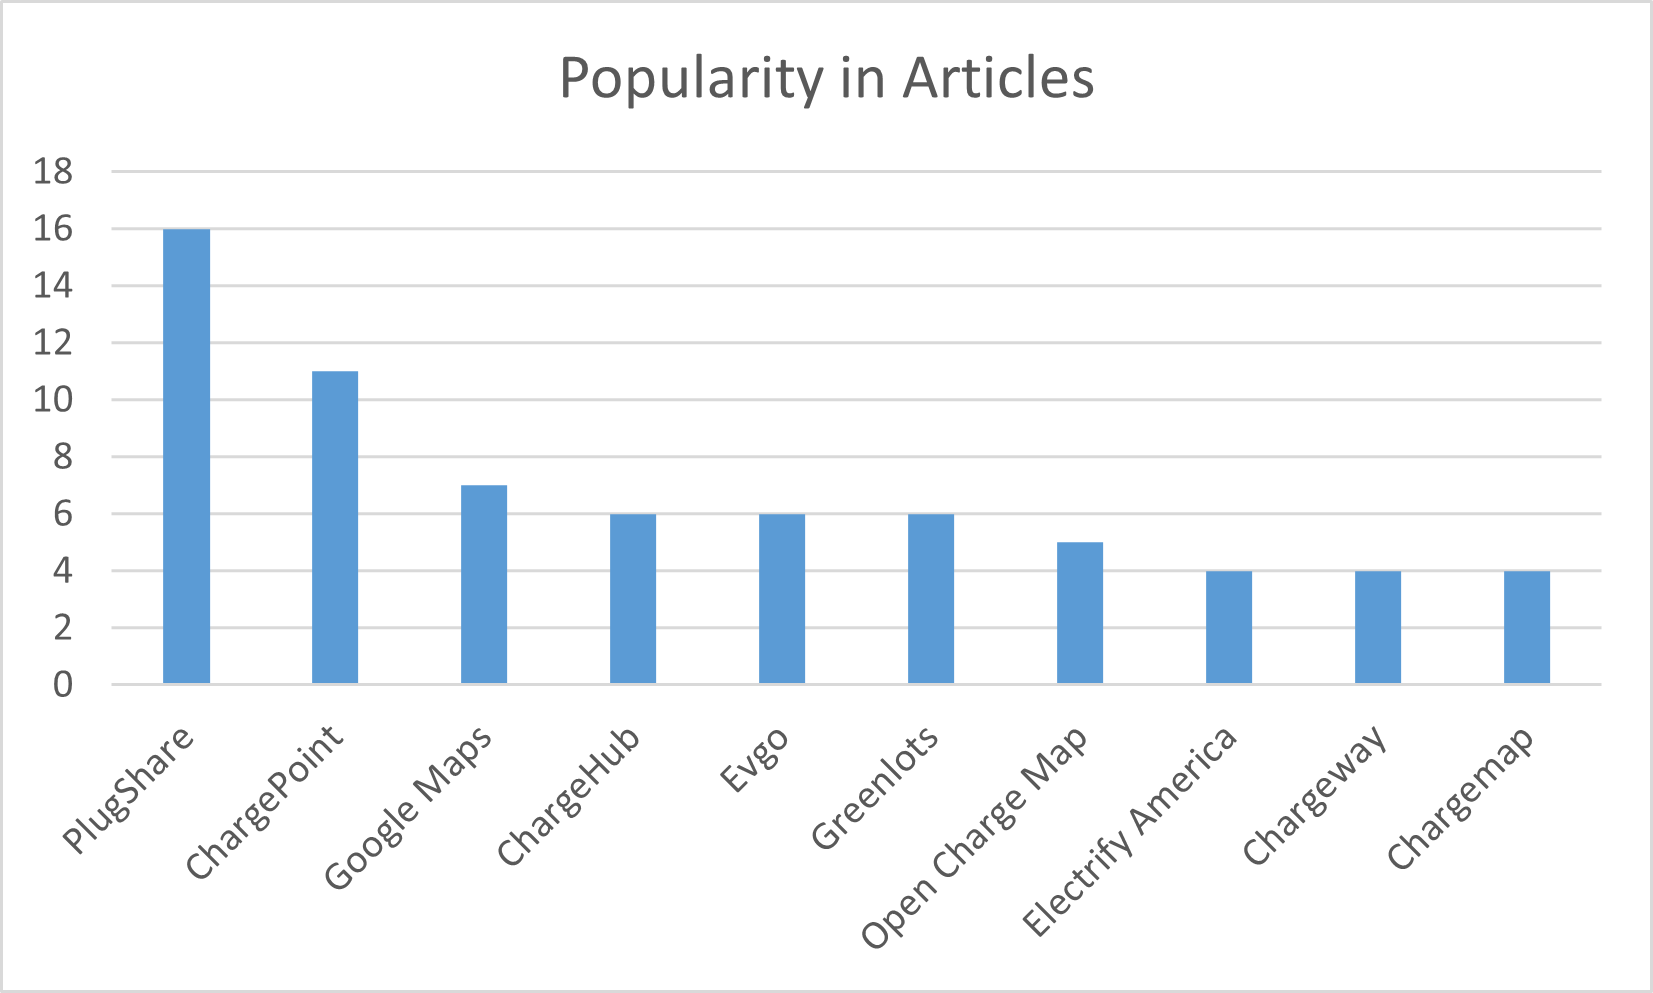
\includegraphics[width=\columnwidth]{Picture5.png}}
\caption{Popularity in Articles}
\label{fig5}
\end{figure}

\begin{table}[htbp]
\caption{Number of Mentions of Website/App}
\begin{center}
\begin{tabular}{|l|r|}
\hline
\multicolumn{1}{|c|}{\textbf{Website/App}} & \multicolumn{1}{c|}{\textbf{Number of Mentions}} \\ \hline
PlugShare & 16 \\
ChargePoint & 11 \\
Google Maps & 7 \\
ChargeHub & 6 \\
Evgo & 6 \\
Greenlots & 6 \\
Open Charge Map & 5 \\
Electrify America & 4 \\
Chargeway & 4 \\
Chargemap & 4 \\ \hline
\end{tabular}
\label{tab4}
\end{center}
\end{table}

\subsection{Popularity based on plugin usage}
There were 20 websites which had plugins from other websites. Only 4 websites provided plugins which could be used in other websites. These websites and the number of websites that use their plugins are listed in ``Table~\ref{tab5}''. PlugShare was again the most popular plugin provider(Fig.~\ref{fig6}).

\begin{figure}[htbp]
\centerline{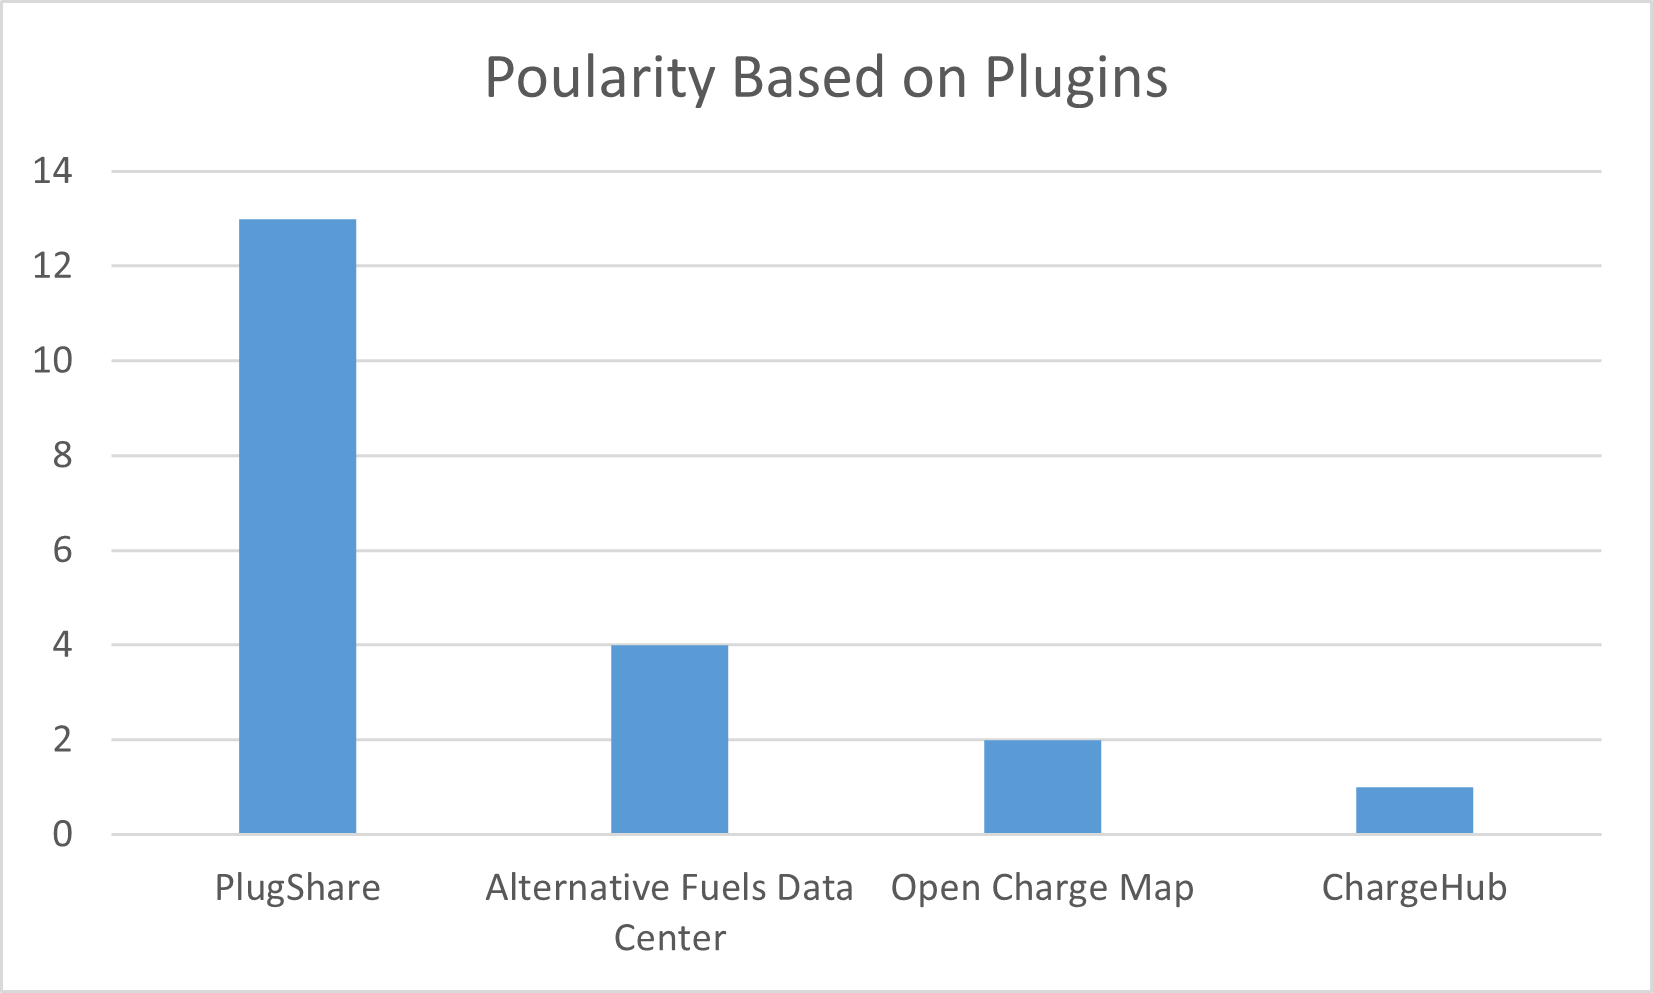
\includegraphics[width=\columnwidth]{Picture6.png}}
\caption{Popularity Based on Plugins}
\label{fig6}
\end{figure}

\begin{table}[htbp]
\caption{Number of Uses of Plugins}
\begin{center}
\begin{tabular}{|l|r|}
\hline
\multicolumn{1}{|c|}{\textbf{Website}} & \multicolumn{1}{c|}{\textbf{Websites with plugins}} \\ \hline
PlugShare & 13 \\
Alternative Fuels Data Center & 4 \\
Open Charge Map & 2 \\
ChargeHub & 1 \\ \hline
\end{tabular}
\label{tab5}
\end{center}
\end{table}

\subsection{Popularity based on App Store ratings}
As the Apple App Store does not provide data on the number of downloads of a particular app we used the next closest metric which could be used to determine the popularity of the app, its ratings and number of ratings. This is based on the assumption that more the people use an app the more they would rate it. PlugShare was again the most highly rated app(Fig.~\ref{fig7}). For comparison the Tesla app, an app made by Tesla, the largest and most popular electric vehicle manufacturer in the USA, has a rating of only 3.8 with 4000 ratings. The list of the top 5 most highly rated apps can be found in ``Table~\ref{tab6}''.

\begin{figure}[htbp]
\centerline{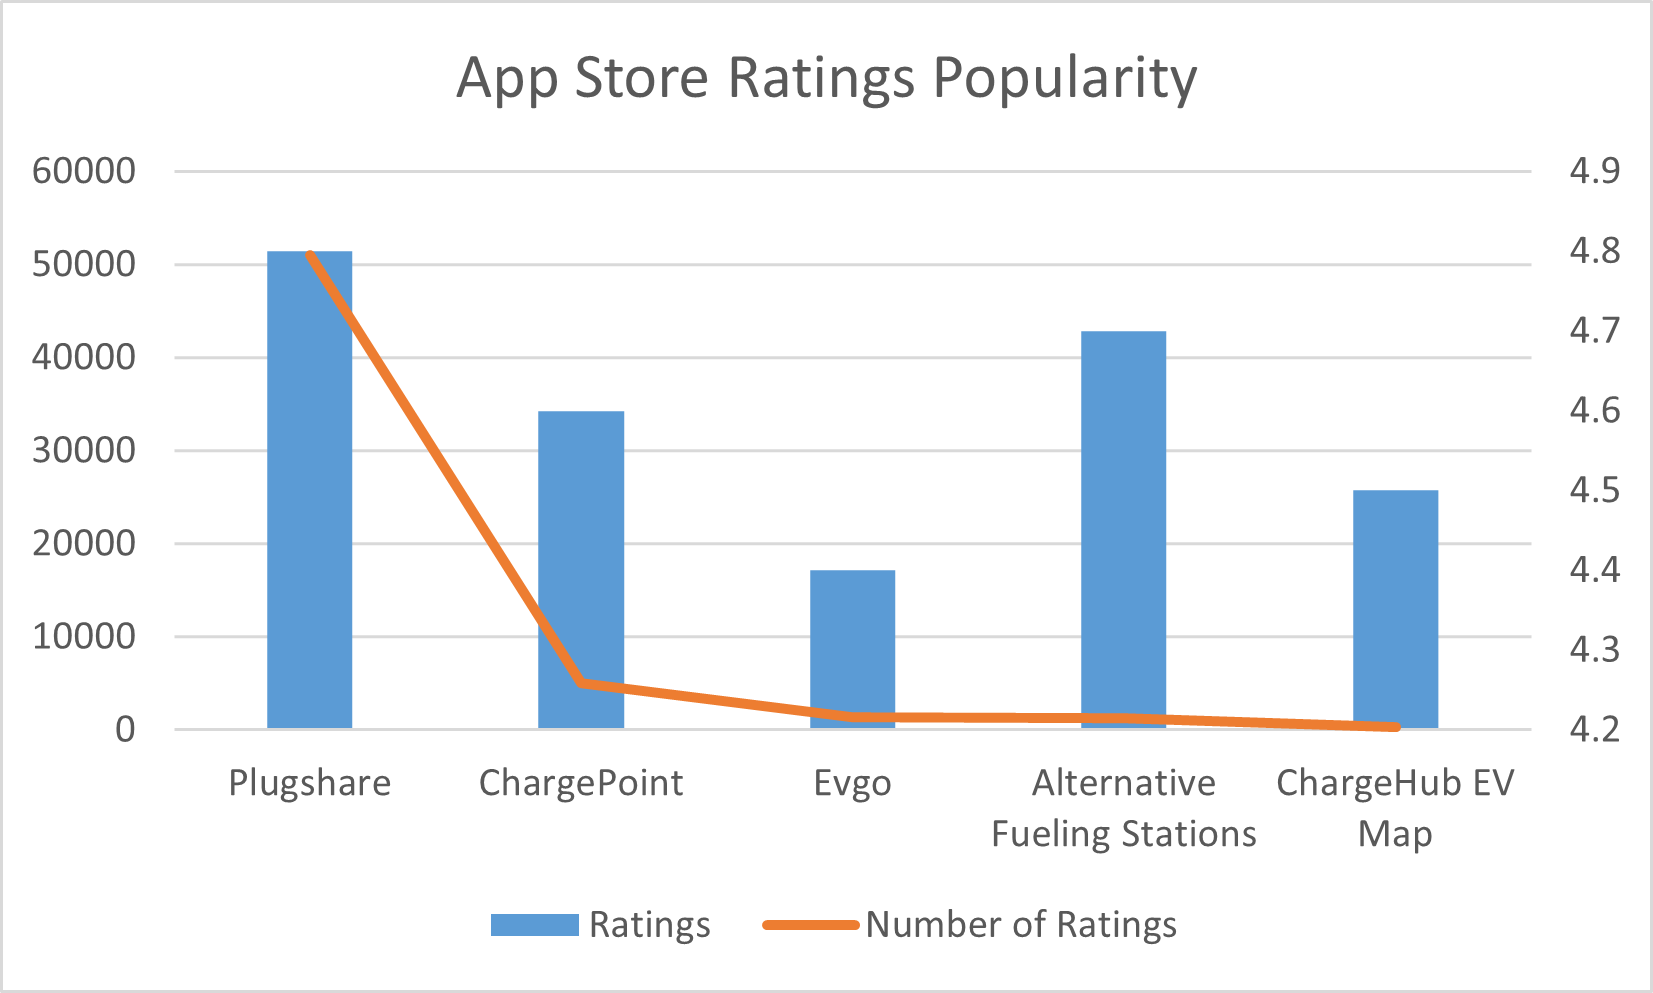
\includegraphics[width=\columnwidth]{Picture7.png}}
\caption{App Store Ratings}
\label{fig7}
\end{figure}

\begin{table}[htbp]
\caption{App Store Ratings}
\begin{center}
\begin{tabular}{|l|l|l|}
\hline
\multicolumn{1}{|c|}{\textbf{App}} & \multicolumn{1}{c|}{\textbf{Rating}} & \multicolumn{1}{c|}{\textbf{Number of Ratings}} \\ \hline
Plugshare & 4.8 & 51000 \\
ChargePoint & 4.6 & 5000 \\
Evgo & 4.4 & 1400 \\
Alternative Fueling Stations & 4.7 & 1300 \\
ChargeHub EV Map & 4.5 & 275 \\ \hline
\end{tabular}
\label{tab6}
\end{center}
\end{table}

\vspace{12pt}
From all the above mentioned analysis we can clearly see that PlugShare is by far the most popular website and app which is used by Electric Vehicle users to find charging stations. The editable attributes for plug share are listed in ``Table~\ref{tab7}''. All these editable attributes in PlugShare are truly editable i.e. they can be edited directly without requiring a review. For comparison all the truly editable attributes of websites/apps with at least one truly editable attribute are listed in ``Table~\ref{tab8}'' along with their type\\

\begin{table*}[htbp]
\caption{PlugShare Truly Editable Attributes}
\begin{center}
\begin{tabular}{|l|l|l|l|l|l|l|l|l|l|l|l|}
\hline
\multicolumn{1}{|c|}{\textbf{Website / App}} & \multicolumn{1}{c|}{\textbf{Address}} & \multicolumn{1}{c|}{\textbf{Parking}} & \multicolumn{1}{p{0.1\columnwidth}|}{\textbf{Plug Type}} & \multicolumn{1}{c|}{\textbf{Price}} & \multicolumn{1}{p{0.12\columnwidth}|}{\textbf{Payment Types}} & \multicolumn{1}{c|}{\textbf{Amenities}} & \multicolumn{1}{p{0.16\columnwidth}|}{\textbf{Operational Status}} & \multicolumn{1}{c|}{\textbf{Timings}} & \multicolumn{1}{c|}{\textbf{Reviews}} & \multicolumn{1}{c|}{\textbf{Photos}} \\ \hline
PlugShare & Yes & Yes & Yes & Yes & No & Yes & No & Yes & Yes & Yes \\ \hline
\end{tabular}
\label{tab7}
\end{center}
\end{table*}

\begin{table*}[htbp]
\caption{Website/App Truly Editable Attributes}
\begin{center}
\begin{tabular}{|l|l|l|l|l|l|l|l|l|l|l|l|}
\hline
\multicolumn{1}{|c|}{\textbf{Website / App}} & \multicolumn{1}{c|}{\textbf{Address}} & \multicolumn{1}{c|}{\textbf{Parking}} & \multicolumn{1}{p{0.1\columnwidth}|}{\textbf{Plug Type}} & \multicolumn{1}{c|}{\textbf{Price}} & \multicolumn{1}{p{0.12\columnwidth}|}{\textbf{Payment Types}} & \multicolumn{1}{c|}{\textbf{Amenities}} & \multicolumn{1}{p{0.16\columnwidth}|}{\textbf{Operational Status}} & \multicolumn{1}{c|}{\textbf{Timings}} & \multicolumn{1}{c|}{\textbf{Reviews}} & \multicolumn{1}{c|}{\textbf{Photos}} & \multicolumn{1}{c|}{\textbf{Type}}  \\ \hline
AFDC & No & No & No & No & No & No & No & No & Yes & No & Crowd Sourced \\
Charge   App & No & No & No & No & No & No & Yes & No & Yes & No & Data Aggregator \\
ChargeHub & No & No & No & No & No & No & No & No & Yes & Yes & Crowd Sourced \\
Chargemap & No & No & No & No & No & No & No & No & Yes & Yes & Crowd Sourced \\
ChargePoint & No & No & No & No & No & No & No & No & Yes & Yes & Charging Network \\
Chargeway & No & No & No & No & No & No & No & No & Yes & Yes & Data Aggregator \\
EVmatch & No & No & No & Yes & No & No & No & No & No & No & Crowd Sourced \\
EVmatch & Yes & Yes & Yes & Yes & Yes & No & Yes & Yes & No & No & Crowd Sourced \\
EVTripMatch & Yes & Yes & Yes & Yes & No & Yes & Yes & Yes & Yes & Yes & Crowd Sourced \\
Google   Maps & No & No & No & No & No & No & Yes & No & Yes & Yes & Crowd Sourced \\
Greenspot & No & No & No & No & No & No & No & No & Yes & No & Charging Network \\
\begin{minipage}[t]{0.17\columnwidth}%
Open Charge Map %
\end{minipage} & No & No & No & No & No & No & No & No & Yes & Yes & Crowd Sourced \\
Plug   Map & Yes & Yes & Yes & Yes & No & No & Yes & Yes & Yes & No & Crowd Sourced \\
PlugShare & Yes & Yes & Yes & Yes & No & Yes & No & Yes & Yes & Yes & Crowd Sourced \\ \hline
\end{tabular}
\label{tab8}
\end{center}
\end{table*}

\section{Security Issues}
The editable attributes in the websites and apps can cause some serious personal and national security issues in the hands of a malicious actor.

\subsection{Cyber attack on the grid}
The grid depends on predictions of usage in order to get power plants inline and offline and to manage supply and demand. Grids can usually deal with gradual rise and fall in supply and demand without any issue. But if there is a sudden spike or drop in demand it can put a lot of pressure on the grid. It can lead to undervolting or overvolting of the grid if the grid can’t react fast enough to the changes. This can also cause a change in the frequency of the grid which can cause severe damage to the grid and anything connected to it. This issue is highlighted in a paper written by Yury Dvorkin titled “Cybersecurity of Smart Electric Vehicle Charging: A Power Grid Perspective” \cite{b2}. This issue can be caused if the pricing, availability and locations of charging networks are edited. This can cause a large number of electric vehicles to gather in a small area to charge themselves. This can cause a sudden spike in demand in the local area and can impact the grid adversely.

\subsection{Damage to infrastructure}
The USA infrastructure is in dire need of repair and upgrades. The American Society of Civil Engineers rates America’s infrastructure as a C-. Bridges in particular receive a rating of C. Currently, 42\% of all bridges are at least 50 years old, and 46,154, or 7.5\% of America's bridges, are considered structurally deficient, meaning they are in “poor” condition. Roads fare worse receiving a rating of D. 40\% of the American road system is in poor or mediocre condition \cite{b3}. This problem will only burgeon with the increase in adoption of electric vehicles. On an average electric vehicles weigh 1 ton more than their non electric counterparts. This is really concerning as the average car weighs 1.5 tons and it represents a 66.66\% increase in the weight of vehicles \cite{b4}. Editing address, plug type, parking, price, availability and plug type could redirect electric vehicle traffic over weak and degraded bridges and roads and can cause damage or collapse of these structures.

\subsection{Personal Safety}
Unlike traditional cars electric vehicles can’t carry extra fuel for emergencies and usually require someone to tow them to a charging point if they run out of charge. As anyone can edit the attributes of a charging station a bad actor could change attributes of certain stations to leave someone stranded in an isolated area or lure someone to an isolated area thus putting the lives of users of these apps at risk. This could be achieved by editing attributes like address, plug type, timings and photos.

\section{Conclusion}
Electric vehicle adoption is going to increase over the next few years as we continue reducing our dependence on fossil fuels. But this change brings along with it new challenges which we have not faced before. We need to revamp our infrastructure to be able to handle the extra loads being put on it by electric vehicles. This includes the electricity, road and bridge related infrastructure. Also ensuring that all the changes which are made to the charging station data on.

\begin{thebibliography}{00}
\bibitem{b1} Gohlke, David, and Zhou, Yan. Assessment of Light-Duty Plug-in Electric Vehicles in the United States, 2010 – 2019. United States: N. p., 2020. Web. doi:10.2172/1642114.
\bibitem{b2} S. Acharya, Y. Dvorkin, H. Pandžić and R. Karri, "Cybersecurity of Smart Electric Vehicle Charging: A Power Grid Perspective," in IEEE Access, vol. 8, pp. 214434-214453, 2020, doi: 10.1109/ACCESS.2020.3041074.
\bibitem{b3} American Society of Civil Engineers, United Sates of America, March 04, 2021. Accessed on: May 10, 2021. [Online]. Available: https://infrastructurereportcard.org/wp-content/uploads/2020/12/National\_IRC\_2021-report.pdf 
\bibitem{b4} Mackenzie, Don \& Zoepf, Stephen \& Heywood, John. (2014). Determinants of USA passenger car weight. Int. J. of Vehicle Design. 65. 73 - 93. 10.1504/IJVD.2014.060066.
\end{thebibliography}
\end{document}
